\subsection{Acceptable coverage}
As motivated in the previous section, a useful library of motion primitives for walking over uneven terrain requires coverage over the start and final configurations of the robot along with a range of kinetic energy additions and subtractions. Depending on the unevenness of the terrain, a diverse range of paths of the end of the swing leg may also be required. All generated constraints should be admissible and usable to avoid wasted memory and computation time.

While it is clear that some density of coverage is required, it is not immediately obvious what constitutes sufficiency. It is advantageous to avoid over-populating the library in order to speed up its generation and real-time use and reduce the memory requirements. However, advantages in computation time are meaningless if the library is insufficient for its purpose. As a result, methods for defining acceptable coverage of the dimensions of this optimisation are required.

\subsubsection{Start and end configurations}
The most important consideration for start and end configuration coverage is to ensure that there is a relatively fine grid of vertical displacements $p_v(\theta^-)$ for a given horizontal displacement to allow for the traversal of the robot over unpredictable terrain. The resolution of this grid and bounds of this grid should be such that the intended terrain is properly discretised; large gaps between the upper/lower bounds and the maximum displacement of the expected terrain should be avoided. Furthermore, the resolution should be fine enough that the large majority of height changes are able to be encoded. As is evident from these requirements, the best choice of grid for height values depends on the terrain for which the library is being designed. We denote the number of unique step heights $n_h$

It is much less important to have a dense grid of horizontal displacements. Indeed, dynamic walking over uneven terrain in most instances achievable with a fixed step length. This fact forms the basis of much of the previous work using feedback-stabilised periodic gaits to enable locomotion over relatively uneven terrain \cite{bigdog?}. Having a small set of step lengths is advantageous in that it enables for intelligent foot placement. Therefore, a small number (less than 10) of horizontal displacements is advisable. Denote the number of unique step lengths $n_l$

Other than in the case of the compass-gait robot, the step length and height are not sufficient to specify the final configuration of the robot. It is therefore necessary to perform inverse kinematics to generate joint angles. In the general case, there are infinitely many combinations of joint angles which can produce the final configuration for a particular step length and height. There is no general method for producing the best configuration; it depends on the robot's mechanical design and the desired gait.  It is not typically necessary to produce multiple final configurations per step length and height on the basis of the terrain interaction alone.

Note that it is essential that the library is designed such that end configurations of virtual constraints match initial configurations of other constraints through the impact map. A primitive is not useful if there are no primitives which can succeed it.

\subsubsection{Inter-step kinetic energy changes}
The only method of velocity control available to the motion planner is to chose constraints which add, maintain or reduce the kinetic energy of the walker. It is therefore important to produce, for each pair of step length and height, a range of kinetic energy mutations. However, producing a fine grid is particularly expensive in this case, since the number of virtual constraints in the library grows $n_ln_h$ members per $\Delta$KE value. It is not of particular importance to the motion planer to have precise control of the velocity, and changes are able to be enacted over several footsteps, therefore a small number of $\Delta$KE values per step length and height is advisable. Denote the number of kinetic energy changes per step length and height $n_k$.

The kinetic energy outcomes of a particular virtual constraint can be used to inform the choice of solution to the inverse kinematics described above. {\color{orange} For the 5-link walker, such and such a method was used}

\subsubsection{Ground configurations}
It is important to consider the likely shape of the ground for constraints with particular step lengths and heights. For the off-line generation of virtual constraints, it is best to be somewhat conservative in specifying where the ground level changes. Consider Figure \ref{fig:stepup}; the terrain steps up at a horizontal displacement significantly smaller than $p_h(\theta^-)$. It is reasonable to expect that this is representative of the typical use case of a step-up virtual constraint. It is not necessary to optimise numerous virtual constraints with varied ground configurations, but with all else fixed. If the terrain profile for the purposes of each single VC optimisation is conservatively defined, the ground configuration is indirectly sampled by producing constraints with varying step length and height.

\begin{figure}
	\centering
	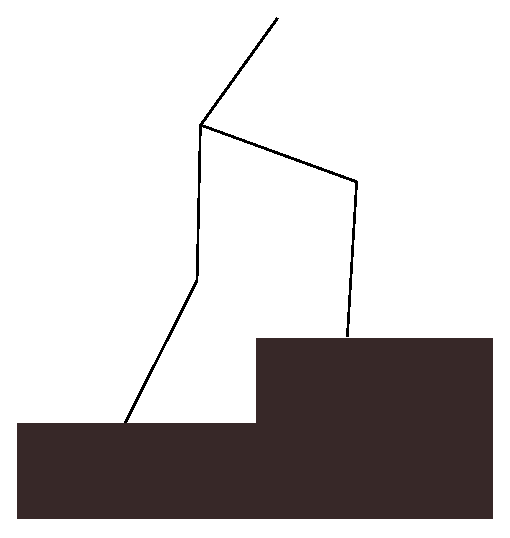
\includegraphics[width=0.5\linewidth]{4VirtConstLib/stepup.eps}
	\caption{Example step-up showing possible terrain profile}
	\label{fig:stepup}
\end{figure}

\subsection{Ordering sets of constraints}
As discussed in Section \ref{sec:primplanning}, planning with primitives is made much more efficient if there is an ordering of primitives, since this facilitates a binary search, reducing the worst-case search time from $O(n)$ to $O(\log n)$. Ordering on the basis of $\Gamma(\theta^\bullet)$ and $\Psi(\theta^\bullet)$

\subsection{Library structure}
Constraints structured together based upon same step length + height, ordering(s) stored, tree/array/linked list/hash table/map?

\subsection{Library generation implementation}
